\section{Ruta 3: Universidad de Ljubljana}

\subsection{Análisis de la ruta obtenida}

Los paquetes hacen varios saltos en Buenos Aires (aunque algunos no responden podemos suponer que son en Buenos Aires), luego de lo cual hay un salto de Buenos Aires a Viena. Esto es anormal, ya que el unico cable submarino que conecta Argentina y Europa llega a España. Esto puede deberse a algún tipo de conexión directa entre Viena y dicho cable. Luego hay algunos saltos mas en Europa hasta llegar a destino. Hay un solo salto intercontinental en el mapa, que es el salto Buenos Aires-Viena, este salto es detectado correctamente, pero al igual que en experimentos anteriores hay muchos falsos positivos.

\subsection{Análisis de las predicciones de salto intercontinental}

\begin{itemize}
	\item Porcentaje de saltos que no responden: 28,57\%
	\item Largo de la ruta de saltos que responden: 10 saltos 
	\item Cantidad de enlaces intercontinentales (separando América del Sur/Norte): 1
	\item Cantidad de outliers: 8
	\item Falsos positivos: 7
	\item Falsos negativos: 0
\end{itemize}

www.uni-lj.si

\begin{figure}[H]
\centering
\begin{tabular}{l | l | l | l | c | c}
Hop & RTT & IP & Ubicación & Predicción de SI & ¿correcto?\\
\hline
1 & 0.0457 & \texttt{192.168.0.1} & Buenos Aires, Argentina & false & \cmark\\
2 & null & null & null & null\\
3 & null & null & null & null\\
4 & null & null & null & null\\
5 & null & null & null & null\\
6 & 0.1651 & \texttt{200.89.161.81} & Buenos Aires, Argentina & true & \xmark\\
7 & 0.3778 & \texttt{200.89.165.86} & Buenos Aires, Argentina & true & \xmark\\
8 & 0.2096 & \texttt{185.70.203.22} & Buenos Aires, Argentina & true & \xmark\\
9 & 0.3915 & \texttt{195.22.215.168} & Viena, Austria & true & \cmark\\
10 & 0.4367 & \texttt{195.22.215.199} & Viena, Austria & false & \cmark\\
11 & 0.5828 & \texttt{77.94.128.25} & Ljubljana, Eslovenia & true & \xmark\\
12 & 0.3733 & \texttt{77.94.139.210} & Ljubljana, Eslovenia & true & \xmark\\
13 & 0.4521 & \texttt{91.216.54.245} & Nova Gorica, Eslovenia & true & \xmark\\
14 & 0.3534 & \texttt{91.223.115.153} & Nova Gorica, Eslovenia & true & \xmark\\
\end{tabular}
\caption{Tabla de resultados para la Universidad de Ljubljana.}
\label{tabla3}
\end{figure}

\begin{figure}[H]
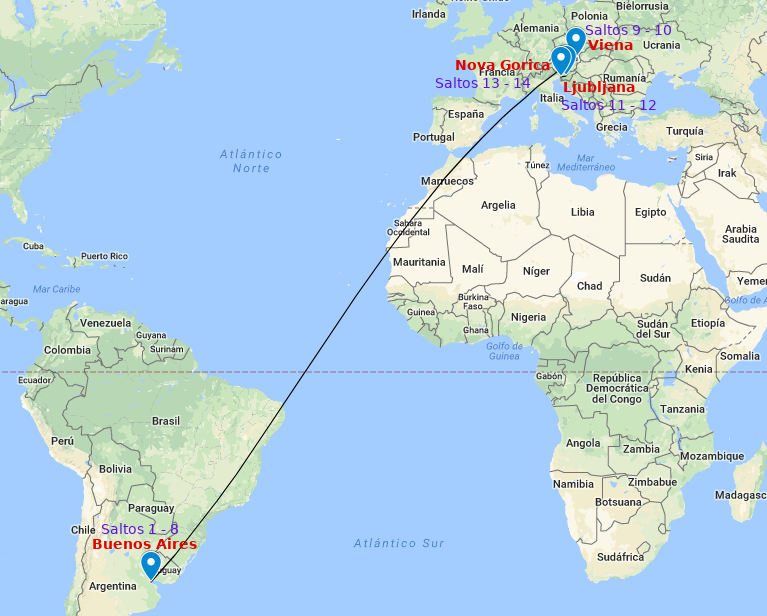
\includegraphics[width=\textwidth]{ljubljana.png}
\caption{Mapa de resultados para la Universidad de Ljubljana.}
\label{mapa3}
\end{figure}

\begin{figure}[H]
\centering
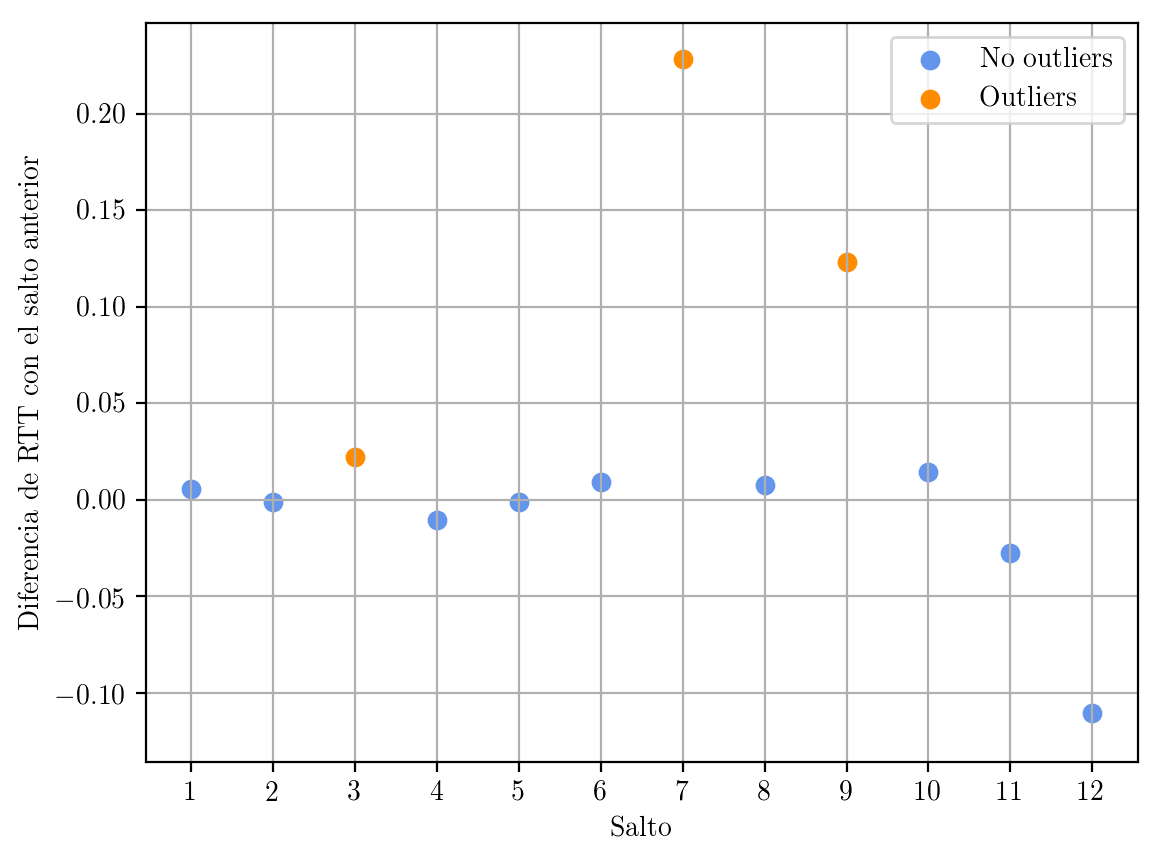
\includegraphics[width=0.6\textwidth]{ljubljana1.png}
\caption{Gráfico de diferencias de RTT en función de cada salto.}
\label{diff3}
\end{figure}

\begin{figure}[H]
\centering
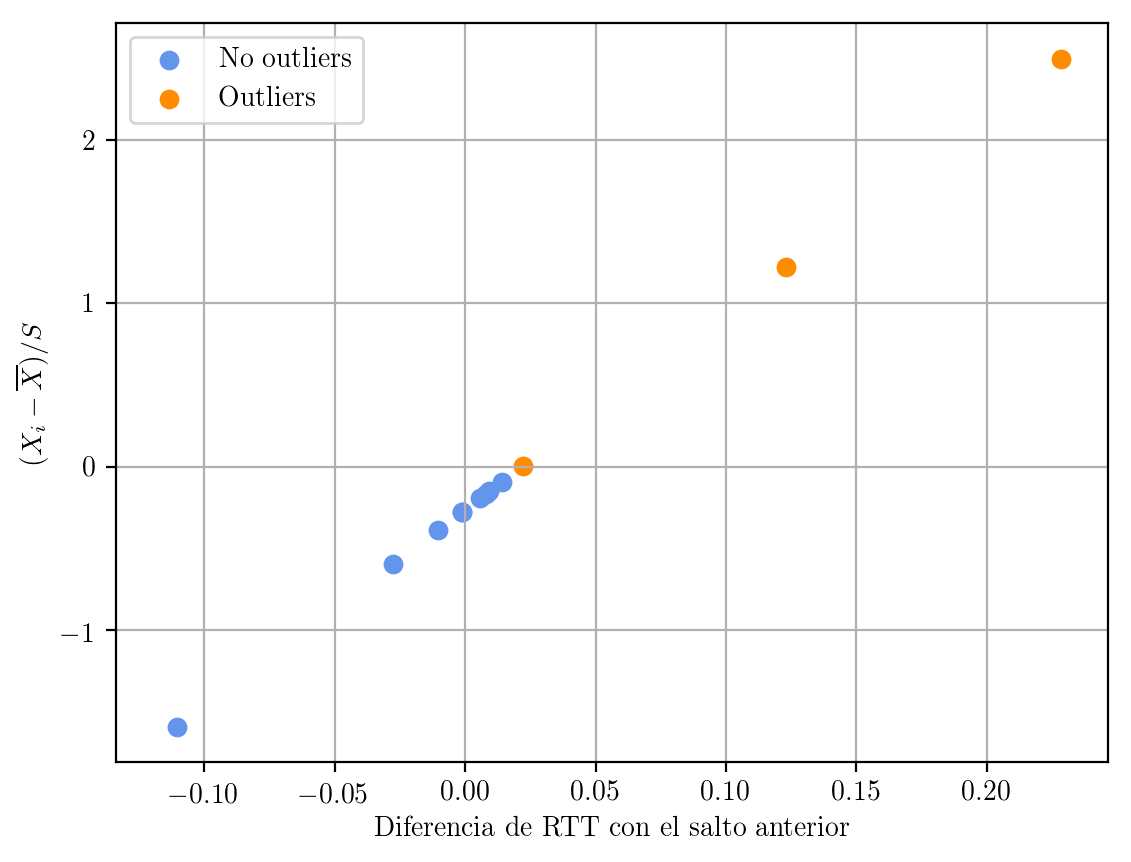
\includegraphics[width=0.6\textwidth]{ljubljana2.png}
\caption{Gráfico de $\frac{X_i - \bar{X}}{S}$ en función de las diferencias de RTT.}
\label{sdev3}
\end{figure}